%% EXERCICIOS PARA INCLUÍR DENTRO DO CADERNO DE EXERCICIOS %%
%
% EXERCICIO.- ANÁLISE DA SECUENCIA: Dies irae
%
\section{Análise da \textit{Chanson} <<A Chantar>>} 
%
Na análise de audición con partitura da música trobadoresca, prestaremos atención fundamentalmente a aspectos como: modo, estilo, ámbito e forma. Como podes observar na figura \ref{fig:a-chantar}, a monodia profana, comparte aspectos de grafía coa música monódica relixiosa.

\par
\vspace*{0.15cm}
%
% ----------------------
% Partitura de audición:
% ----------------------
\begin{figure}[h]
    \centering
    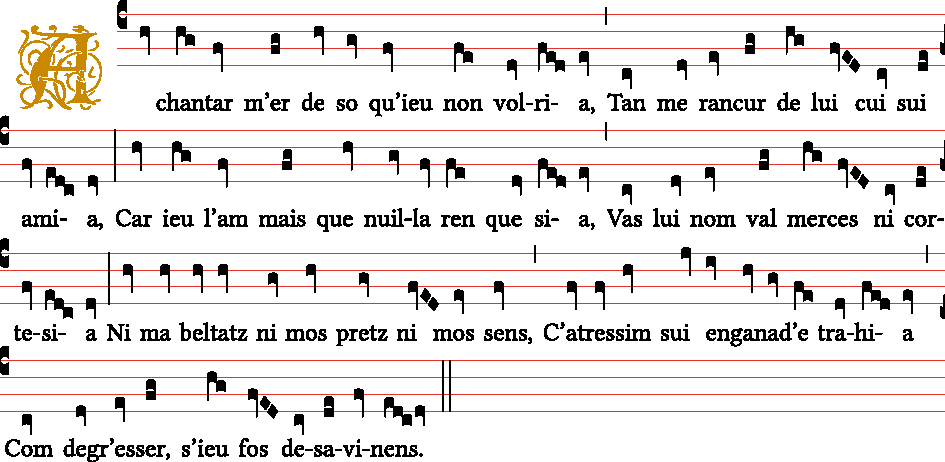
\includegraphics[width=0.80\textwidth]{figures/audicions/A-Chantar.pdf}
    \caption{Melodía e texto da \textit{Chanson} <<A Chantar>> da condesa Beatrix de Dia.}
    \label{fig:a-chantar}
\end{figure}
% -----------------------
%
\subsection*{Indicacións para realizar a análise}
%
\begin{multicols}{2}
%
[Prestaremos atención aos seguintes puntos para realizar a análise e resumo das características:
]
\subsubsection*{Modo}

No repertorio trobadoresco --e na monodia profana, polo xeral-- empregaremos os nomes de orixe da teoría musical grega: \textit{dórico}, \textit{frixio}, \textit{lidio} e \textit{mixolidio}. Os nomes eclesiásiticos e os números de modo empréganse no canto litúrxico.

\subsubsection*{Estilo do canto}

Diferenciamos tan só os estilos \textbf{silábico} e \textbf{ornamentado}. Teremos en conta que estas cancións non estarán únicamente nun estilo senón que oscilan entre ámbolos dous; indicaremos entón o predominante e a diferencia entre versos ou seccións.

\subsubsection*{Ámbito}

Indicaremos o intervalo total entre a nota máis grave e a máis aguda, asi como a distancia de ámbalas dúas á nota final. Debemos indicar tamén as diferencias de ámbito entre seccións ou versos.

\subsubsection*{Estrutura formal}

No caso de ter texto completo, indicaremos o número total de estrofas e a presencia de \textit{tornada}.

Prestaremos atención á liña melódica de cada verso da estrofa e crearemos un esquema asignando diferenes letras a melodías diferentes.
Se a estrofa se divide en seccións, indicarémolo igualmente.
\par
\vspace*{0.3cm}
\newpage
%
    \begin{enumerate}[1.-]
% ANÁLISE DO RITMO DA OBRA:
        \item % RITMO
        \textbf{Ritmo}. Identificamos o ritmo, tendo en conta: pulso, indicacións de compás e outras indicacións dinámicas. 
        Neste caso, estamos ante un ritmo:
        \begin{enumerate}[a)]
            \item mensural 
            \item non mensural 
        \end{enumerate}
% ANÁLISE DA MELODÍA DA OBRA:
        \item %MELODÍA:
        \textbf{Melodía}. Tendo en conta a melodía, determinamos o modo, ámbito e estilo. Prestaremos atención ao perfil melódico e interválica, observando se hai grandes saltos ou mais ben discorre por graos conxuntos.
%        \begin{multicols}{2}
        \begin{enumerate}[a)]
            \item 
            Que intervalos se repiten con maior frecuencia? \dotfill
            \item 
            Cal é o maior intervalo que podemos atopar na peza? \dotfill
            \item
            Podemos afirmar que a melodía se move por graos \dotfill
        \end{enumerate}
%        \end{multicols}
        Vexamos a continuación o Modo, Ámbito e Estilo tendo en conta a melodía:
        \begin{itemize}
% ANÁLISE DO MODO:
            \item % MODO
            \textbf{Modo}.
        \begin{itemize}            
            \item 
            Identifica a clave \dotfill
            \item 
            Cal é a nota final? \dotfill
            \item
            Cal é a nota tenor? \dotfill 
%            \item
%            En que modo básico estamos? \dotfill
            \item
            Cal é a nota máis agura? \dotfill 
            \item
            Cal é a nota máis grave? \dotfill 
            \item
            Que intervalo forman? \dotfill
            \item
            Que intervalo forma a máis aguda coa final? \dotfill
            \item
            Que intervalo forma a máis grave coa final? \dotfill 
            \item
            En qué modo esta a obra? \dotfill
       \end{itemize}
% ANÁLISE DO ÁMBITO DA OBRA:
            \item % ÁMBITO
            \textbf{Ámbito}. \\
            Fixándonos na nota final e na máis aguda:
                \begin{itemize}
                    \item
                    Que intervalo forman? \dotfill
                    \item
                    A melodía é de ámbito dunha \dotfill
                \end{itemize}
            \item % ESTILO
            \textbf{Estilo do canto}. \\ Segundo a relación musica-texto, estamos ante un estilo:
                \begin{enumerate}[a)]
                  \item
                  Silábico \dotfill
                  \item
                  Ornamentado \dotfill
%                  \item
%                  Melismático \dotfill
                \end{enumerate}
        \end{itemize}
        \item % TIMBRE
        \textbf{Timbre}. \\
        Segundo as características da obra, debemos diferenciar as voces, instrumentos, formacións, agrupacións, ...
            \begin{itemize}
                \item 
                Que timbres recoñeces? \dotfill
                \item
                Quen leva a melodía principal? \dotfill
            \end{itemize}
% ANÁLISE DA TEXTURA DA OBRA:
        \item %TEXTURA
        \textbf{Textura}. \\
        Polas características da obra, diferenciamos unha textura melódica de escrita\ldots 
            \begin{enumerate}[a)]
                \item 
                horizontal, monódica en heterofonía
                \item 
                horizontal, polifónica en heterofonía
            \end{enumerate}
% ANÁLISE DA FORMA DA OBRA
        \item %FORMA:
        \textbf{Estrutura formal}. \\
        Determinamos a forma segundo a textura e estrutura da obra.
%        \par %Pregunta sobre as Formas
            \begin{enumerate}[a)]
                \item
                Cantos versos diferencias na peza? \dotfill
                \item
                Que versos teñen igual melodía? \dotfill
                \item
                Cales teñen melodía diferente? \dotfill
                \end{enumerate}
%
        \begin{enumerate}[a)]
            \item 
            Forma vocal menor libre
            \item
            Forma vocal menor ternaria
            \item
            Forma vocal maior ternaria
            \item
            Forma instrumental menor ternaria
        \end{enumerate}
        \end{enumerate}
%    \end{multicols}
%
\end{multicols}
%\vspace*{0.25cm}
%
\subsubsection*{Clasificación no repertorio} \label{Clasificación-dies-irae}
Unha vez realizada a análise da audición, tendo en conta os datos obtidos, clasificaremos a obra tendo en conta sobre todo o ámbito e estilo.
%
% RESUMO DA AUDICIÓN DO EXERCICIO
%
\vspace*{0.5cm}
\begin{ejercicio}[Características principais da audición: <<Dies irae>>]
%\small{
%Redacta un breve comentario da obra. Ten en conta a análise feita:
%}

% ESPACIO PARA REDACTAR O COMENTARIO DA AUDICIÓN
%
%\small{Trátase dunha forma vocal menor, de estrutura ternaria; segundo o ámbito e estilo, obedece a un canto antifonal do propio da misa cantado a capella por un coro de voces masculinas; a textura monódica horizontal é propia do canto chá (Gregoriano) en estilo neumático na primeira sección e silábico na segunda, de ámbito reducido escrita no modo \textit{tetrardus auténtico} (VII)     }

        \vspace*{2.78cm}
\end{ejercicio}

